\documentclass[epsfig,10pt,fullpage]{article}

\newcommand{\LabNum}{3}
\newcommand{\CommonDocsPath}{../../common/docs}
\addtolength{\textwidth}{1.5in}
\addtolength{\oddsidemargin}{-0.75in}
\addtolength{\topmargin}{-0.75in}
\addtolength{\textheight}{1.5in}
\addtolength{\evensidemargin}{0.75in}
\setlength\parindent{0pt}
\raggedbottom

\usepackage{ae,aecompl}
\usepackage{epsfig,float,times}
\usepackage[hypcap]{caption}
\usepackage[pdftex, colorlinks]{hyperref}
\usepackage{graphicx}
\usepackage[usenames, dvipsnames]{color}
\usepackage{rotating}
\usepackage{tikz}
\usetikzlibrary{automata,positioning}
\usepackage{placeins}

\widowpenalty 10000
\clubpenalty 10000

\newcommand{\red}[1]{{\color{red}\sf{#1}}}
\newcommand{\green}[1]{{\color{green}\sf{#1}}}
\newcommand{\blue}[1]{{\color{blue}\sf{#1}}}
\definecolor{PineGreen}{rgb}{0.0, 0.47, 0.44}
\definecolor{ForestGreen}{rgb}{0.13, 0.55, 0.13}
\definecolor{Brown}{rgb}{0.59, 0.29, 0.0}

\newcommand{\UPDatePublished}{Oct 2021}
\newcommand{\versnum}{21.1} %version number quartus/AMP
\newcommand{\quartusname}{Quartus\textsuperscript{\textregistered} Prime}	
\newcommand{\UPTextBar}{For \quartusname{} \versnum{}}
\newcommand{\thisyear}{2021 } %for copyright
\newcommand{\company}{FPGAcademy.org}
\newcommand{\longteamname}{FPGAcademy.org}
\newcommand{\teamname}{FPGAcademy}
\newcommand{\website}{FPGAcademy.org}

\newcommand{\productAcronym}{AMP}
\newcommand{\productNameShort}{Monitor Program}

\newcommand{\productNameMedTM}{A Monitor Program}
\newcommand{\productNameMed}{A Monitor Program}

%\newcommand{\headerLogoFilePath}[1]{#1/FPGAcademy.png}

% listings is a package that supports encapsulating source code in LaTeX conveniently
\usepackage{listings}

\def\expandparam\lstinputlisting[#1]#2{\edef\tmp{\noexpand\lstinputlisting[#1]{#2}}\tmp}

%%%%%%%%%%%%%%%%%%%% Source Code Formatting %%%%%%%%%%%%%%%%%%%%
\definecolor{globalCommentColour}{rgb}{0.588,0.588,0.588}

%%%%%%%%%%%%%%%%%%%%%%%%%%%%%%%%%%%%%%%%%%%%%%%%%%%%
% Defining language style
% NiosII ASM
\lstdefinelanguage[NiosII]{Assembler} {
  morekeywords={add, addi, and, andhi, andi, beq, bge, bgeu, bgt, bgtu, ble,  bleu, blt, bltu, bne, br, break,% 
  bret, call, callr, cmpeq, cmpeqi, cmpge, cmpgei, cmpgeu, cmpgeui, cmpgt, cmpgti, cmpgtu, cmpgtui, cmple,%
  cmplei, cmpleu, cmpleui, cmplt, cmplti, cmpltu, cmpltui, cmpne, cmpnei, custom, div, divu, eret, flushd,%
  flushda, flushi, flushp, initd, initda, initi, jmp, jmpi, ldb, ldbio, ldbu, ldbuio, ldh, ldhio, ldhu, ldhuio,%
  ldw, ldwio, mov, movhi, movi, movia, movui, mul, muli, mulxss, mulxsu, mulxuu, nextpc, nop, nor, or, orhi, ori,%
  rdctl, rdprs, ret, rol, roli, ror, sll, slli, sra, srai, srl, srli, stb, stbio, sth, sthio, stw, stwio,%
  sub, subi, sync, trap, wrctl, wrtcl, wrprs, xor, xori, xorhi, xori},% 	
  morekeywords=[2]{.abort, .ABORT, .align, .app-file, .ascii, .asciz, .balign, .byte, .comm, .data, .def,%
  .desc, .dim, .double, .eject, .else, .end, .endef, .endif, .equ, .equiv, .err, .extern, .file, .fill, .float,%
  .global, .globl, .hword, .ident, .if, .include, .int, .irp, .irpc, .lcomm, .lflags, .line, .linkonce, .ln,%
  .list, .long, .macro, .mri, .nolist, .octa, .org, .p2align, .psize, .quad, .rept, .sbttl, .scl, .section,%
  .set, .short, .single, .size, .sleb128, .skip, .space, .stadb, .stabn, .stabs, .string, .symver, .tag,%
  .text, .title, .type, .val, .uleb128, .word},% 	
  morekeywords=[3]{et, bt, gp, sp, fp, ea, sstatus, ra, pc, status, estatus, bstatus, ienable, ipending, cpuid,%
  exception, pteaddr, tlbacc, tlbmisc, eccinj, badaddr, config, mpubase, mpuacc},% 	
  sensitive=t,%
  alsoletter=.,%
  morestring=[b]",%
  morecomment=[s]{/*}{*/},%
  morecomment=[l]\#,%
}[keywords,comments,strings]
   
%% NOTE: morekeywords=[2] are GNU directives.
   
\definecolor{niosInstructionColour}{rgb}{0.000,0.608,0.000}
\definecolor{niosDirectiveColour}{rgb}{0.000,0.000,0.902}
\definecolor{niosSpecialRegColour}{rgb}{0.000,0.000,0.000}
\definecolor{niosStringColour}{rgb}{0.808,0.482,0.000}
   
%% NOTE: To make bold use: =\bfseries\color{<colour>}
\lstdefinestyle{defaultNiosStyle} {
  language=[NiosII]{Assembler},
  stringstyle=\color{niosStringColour},
  keywordstyle=\color{niosInstructionColour},
  keywordstyle=[2]\color{niosDirectiveColour},
  keywordstyle=[3]\itshape\color{niosSpecialRegColour}
}
%%%%%%%%%%%%%%%%%%%%%%%%%%%%%%%%%%%%%%%%%%%%%%%%%%%%

%%%%%%%%%%%%%%%%%%%%%%%%%%%%%%%%%%%%%%%%%%%%%%%%%%%%
% Defining language style
% ArmA9 ASM
\lstdefinelanguage[ArmA9]{Assembler} {
  morekeywords={ADC, ADD, ADDS, AND, ANDS, B, BAL, BEQ, BGE, BGT, BL, BLT, BIC, BKPT, BLX, BNE, BX, CDP, CLZ, CMN, CMP, EOR,%
  EORS, LDC, LDM, LDR, LDRB, LDRBT, LDRH, LDRSB, LDRSH, LDRT, LSL, MCR, MLA, MOV, MOVW, MOVT, MRC, MRS, MSR, MUL, MVN, ORR, PLD,%
  ROR, RSB, RSC, SBC, SMLAL, SMULL, STC, STM, STR, STRB, STRBT, STRH, STRT, SUB, SUBS, SWI, SWP, SWPB, TEQ, UMLAL,
  PUSH, POP, MOVS, RORS, LSR},%
  morekeywords=[2]{.abort, .ABORT, .align, .app-file, .ascii, .asciz, .balign, .byte, .comm, .data, .def,%
  .desc, .dim, .double, .eject, .else, .end, .endef, .endif, .equ, .equiv, .err, .extern, .file, .fill, .float,%
  .global, .globl, .hword, .ident, .if, .include, .int, .irp, .irpc, .lcomm, .lflags, .line, .linkonce, .ln,%
  .list, .long, .macro, .mri, .nolist, .octa, .org, .p2align, .psize, .quad, .rept, .sbttl, .scl, .section,%
  .set, .short, .single, .size, .sleb128, .skip, .space, .stadb, .stabn, .stabs, .string, .symver, .tag,%
  .text, .title, .type, .val, .vectors, .uleb128, .word},%
  morekeywords=[3]{SP, PC, MIDR, CTR, TCMTR, TLBTR, MPIDR, ID_PFR0, ID_PFR1, ID_DFR0, ID_MMFR0, ID_MMFR1, ID_MMFR2,%
  ID_MMFR3, ID_ISAR0, ID_ISAR1, ID_ISAR2, ID_ISAR3, ID_ISAR4, CCSIDR, CLIDR, AIDR, CSSELR, TTBR0, TTRB1, TTBR2, DACR,%
  DFSR, IFSR, ADFSR, AIFSR, DFAAR, IFAR, ICIALLUIS, BPIALLIS, PAR, ICIALLU, ICIMVAU, BPIALL, DCIMVAC, DCISW, V2PCWPR,%
  DCCVAC, DCCSW, DDIMVAC, DCISW, TLBALLIS, TLBIMVAIS, TLBIASIDIS, TLBIMVAAIS, TLBIALL, TLBIMVA, TLBIASID, TLBIMVAA,%
  PMCR, PMCNTENSET, PMCNTENCLR, PMOVSR, PMSWINC, PMSELR, PMXEVTYPER, PMXEVCNTR, PMUSERENR, PMINTENSET, PMINTENCLR,%
  PRRR, NRRR, PLEIDR, PLEASR, PLEFSR, PLEUAR, PLEPCR, VBAR, MVBAR, ISR, FCSEIDR, CONTEXTIDR, TPIDRURW, TPIDRURO, TPIDRPRW},%
  sensitive=f,%
  alsoletter=.,%
  morestring=[b]",%
  morecomment=[s]{/*}{*/},%
  morecomment=[l]{//},%
}[keywords,comments,strings]
   
%% NOTE: morekeywords=[2] are GNU directives.
   
\definecolor{armInstructionColour}{rgb}{0.000,0.608,0.000}
\definecolor{armDirectiveColour}{rgb}{0.000,0.000,0.902}
\definecolor{armSpecialRegColour}{rgb}{0.000,0.000,0.000}
\definecolor{armStringColour}{rgb}{0.808,0.482,0.000}
   
\lstdefinestyle{defaultArmStyle} {
  language=[ArmA9]{Assembler},
  stringstyle=\color{armStringColour},
  keywordstyle=\color{armInstructionColour},
  keywordstyle=[2]\color{armDirectiveColour},
  keywordstyle=[3]\itshape\color{armSpecialRegColour}
}
%%%%%%%%%%%%%%%%%%%%%%%%%%%%%%%%%%%%%%%%%%%%%%%%%%%%

%%%%%%%%%%%%%%%%%%%%%%%%%%%%%%%%%%%%%%%%%%%%%%%%%%%%
% Defining language style
% FPGAcademy ASM
\lstdefinelanguage{ASM}{
  morekeywords = [1]{mv, mvt, mvne, mvcc, add, sub, st, ld, and, b, bne, beq, bcc, bcs},
  morekeywords = [2]{word, define},
  keywordstyle = [1]\color{ForestGreen},
  keywordstyle = [2]\color{blue},
  sensitive = true,
  morecomment = [l]{//},
}

\lstset{
  language = ASM,
  basicstyle=\small\color{black}\ttfamily,
  commentstyle=\small\color{Brown}\itshape\ttfamily,
  showstringspaces=false,
  frame=none, %lines % boxed listings
  breaklines=true,
  breakatwhitespace=true,
  tabsize=3
}
%%%%%%%%%%%%%%%%%%%%%%%%%%%%%%%%%%%%%%%%%%%%%%%%%%%%

%%%%%%%%%%%%%%%%%%%%%%%%%%%%%%%%%%%%%%%%%%%%%%%%%%%%
% Defining language style
% Java
\definecolor{javaStringColour}{rgb}{0.808,0.482,0}
%%%%%%%%%%%%%%%%%%%%%%%%%%%%%%%%%%%%%%%%%%%%%%%%%%%%

%%%%%%%%%%%%%%%%%%%%%%%%%%%%%%%%%%%%%%%%%%%%%%%%%%%%
% Defining language style
% C
\definecolor{CStringColour}{rgb}{0.808,0.482,0}

\lstset{
  language = C,
  basicstyle=\small\color{black}\ttfamily, 
  commentstyle=\small\color{PineGreen}\itshape\ttfamily,
  keywordstyle=\small\color{blue}\bfseries\ttfamily,
  showstringspaces=false,
  frame=none, %lines % boxed listings
  breaklines=true,
  breakatwhitespace=true,
  tabsize=3
}
%%%%%%%%%%%%%%%%%%%%%%%%%%%%%%%%%%%%%%%%%%%%%%%%%%%%

%%%%%%%%%%%%%%%%%%%%%%%%%%%%%%%%%%%%%%%%%%%%%%%%%%%%
% Defining language style
% Verilog
\definecolor{verilogCommentColour}{rgb}{0.000,0.502,0.000}

\lstdefinestyle{defaultVerilogStyle} {
  language={Verilog},
  keywordstyle=\color{blue},
  commentstyle=\color{verilogCommentColour}
}
%%%%%%%%%%%%%%%%%%%%%%%%%%%%%%%%%%%%%%%%%%%%%%%%%%%%

%%%%%%%%%%%%%%%%%%%%%%%%%%%%%%%%%%%%%%%%%%%%%%%%%%%%
% Defining language style
% VHDL
\lstdefinestyle{defaultVHDLStyle} {
  language={VHDL},
  keywordstyle=\color{blue},
  commentstyle=\color{verilogCommentColour}
}
%%%%%%%%%%%%%%%%%%%%%%%%%%%%%%%%%%%%%%%%%%%%%%%%%%%%

%%%%%%%%%%%%%%%%%%%%%%%%%%%%%%%%%%%%%%%%%%%%%%%%%%%%
% Defining language style
% LaTeX
\lstdefinelanguage[LocalLaTeX]{TeX}[LaTeX]{TeX}{moretexcs={bf, it, sf, lstset},}

\lstdefinestyle{defaultLocalLatexStyle} {
  language=[LocalLatex]{TeX},
  keywordstyle=\color{blue}\bfseries,
  keywordstyle=[2]\color{blue},
  keywordstyle=[3]\color{blue}\bfseries
}
%%%%%%%%%%%%%%%%%%%%%%%%%%%%%%%%%%%%%%%%%%%%%%%%%%%%

%%%%%%%%%%%%%%%%%%%%%%%%%%%%%%%%%%%%%%%%%%%%%%%%%%%%
% Defining language style
% Default
\lstset{
  basicstyle=\small\color{black}\ttfamily,
  commentstyle=\small\color{globalCommentColour}\itshape\ttfamily,
  keywordstyle=\small\color{blue}\bfseries\ttfamily,
  showstringspaces=false,
  frame=none, %lines % boxed listings
  breaklines=true,
  breakatwhitespace=true,
  tabsize=3
}
%%%%%%%%%%%%%%%%%%%%%%%%%%%%%%%%%%%%%%%%%%%%%%%%%%%%


\hypersetup{
  pdftitle={OPAE Lab Exercise \LabNum},
  linkcolor=blue,
  hyperindex=true,
  pdfauthor={FPGAcademy.org},
  pdfkeywords={FPGAcademy.org, FPGAcademy, Lab, Exercise, OPAE},
  bookmarks,
  bookmarksopen=false,
  filecolor=blue,
  pdfstartview={FitH},
  urlcolor=blue,
  plainpages=false,
  pdfpagelabels=true,
  linkbordercolor={1 1 1} %no color for link border
}



\begin{document}

\centerline{\huge OPAE}
~\\
\centerline{\huge Laboratory Exercise \LabNum}
~\\
\centerline{\large Streaming Direct Memory Access (DMA)}
~\\

\noindent
This exercise shows how to design a streaming Direct Memory Access(DMA) Accelerator Functional Unit(AFU). \\
\\
To complete this exercise you need to be familiar with the Platform Designer in the Intel Quartus Prime software, which is used in the design of the AFU hardware, and the C++ programming language, which is used to write the software program that make use of the AFU.\\
\\
The exercise is organized into the following stages:
\begin{enumerate}
    \item Create a streaming DMA AFU which performs edge detection. In this step, you will augment a basic streaming DMA sytem which only performs data transfers with the edge detection component.
    \item Design a software application that utilize the streaming DMA AFU. 
\end{enumerate}


\section*{Part I}
Figure \ref{fig:diagram} provides a high-level block diagram of a DMA AFU. It communicates with the FPGA Interface Unit(FIU) with the {\it Core Cache Interface} protocol (CCI-P). The MMIO Decoder Logic then separates Memory-Mapped IO(MMIO) and the DMA read and write channels. We will use MMIO for control and status signals and the DMA channels for transferring data between the processor and the AFU.\\

\begin{figure}[h]
    \centering
    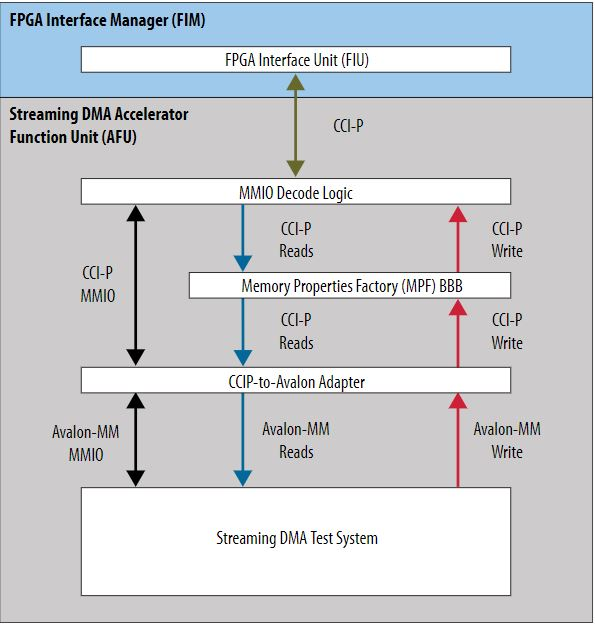
\includegraphics[width=0.5\textwidth]{figures/diagram_dmast.JPG}
    \caption{A block diagram}
    \label{fig:diagram}
\end{figure}

\noindent
For this exercise, we will use an Avalon Memory Mapped interface for the application logic circuit. As shown in Figure \ref{fig:diagram}, the CCI-P to Avalon-MM Adapter converts the CCI-P interface to the Avalon-MM interface. A Memory Properties Factory(MPF) module is added between the MMIO Decoder Logic and the CCI-P to Avalon-MM Adapter. This module ensures that read responses from the DMA return in the order that they were issued, which is required by the Avalon-MM protocol.\\


\noindent
Figure \ref{fig:qsys} illustrates a basic streaming DMA system. The M2S DMA BBB reads data from memory and provides the data as a serial stream while the S2M DMA BBB accepts a serial stream of data and writes the data back to memory. The CSR Pipeline Bridge is connected to the MMIO channel. The Host Read Pipeline Bridge and the Host Write Far Reach Bridge are connected to the DMA read channel and write channel, respectively. The EMIF Clock Crossing Bridges are connected to the local memory of the FPGA. For this exercise, we will only transfer data to and from the processor through the host write/read bridges and will not use the local memory of the FPGA.\\

\begin{figure}[h]
    \centering
    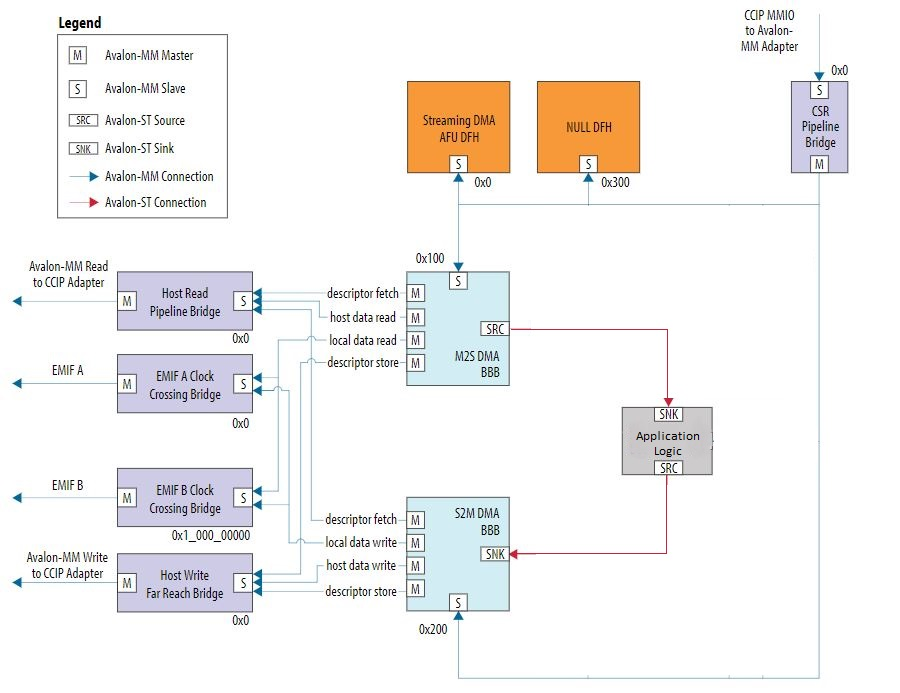
\includegraphics[width=0.7\textwidth]{figures/streaming_AFU.jpg}
    \caption{streaming DMA system}
    \label{fig:qsys}
\end{figure}

\noindent
The streaming DMA system and the M2S DMA BBB and the S2M DMA BBB subsystems each has a device feature headers(DFH). A DFH contains information of a system which allows the processor to identify the system. The Streaming DMA AFU DFH in Figure \ref{fig:qsys} is the DFH of the AFU. It includes the {\it universally unique identifier} (UUID) for the AFU.\\
\\
\begin{figure}[h]
    \centering
    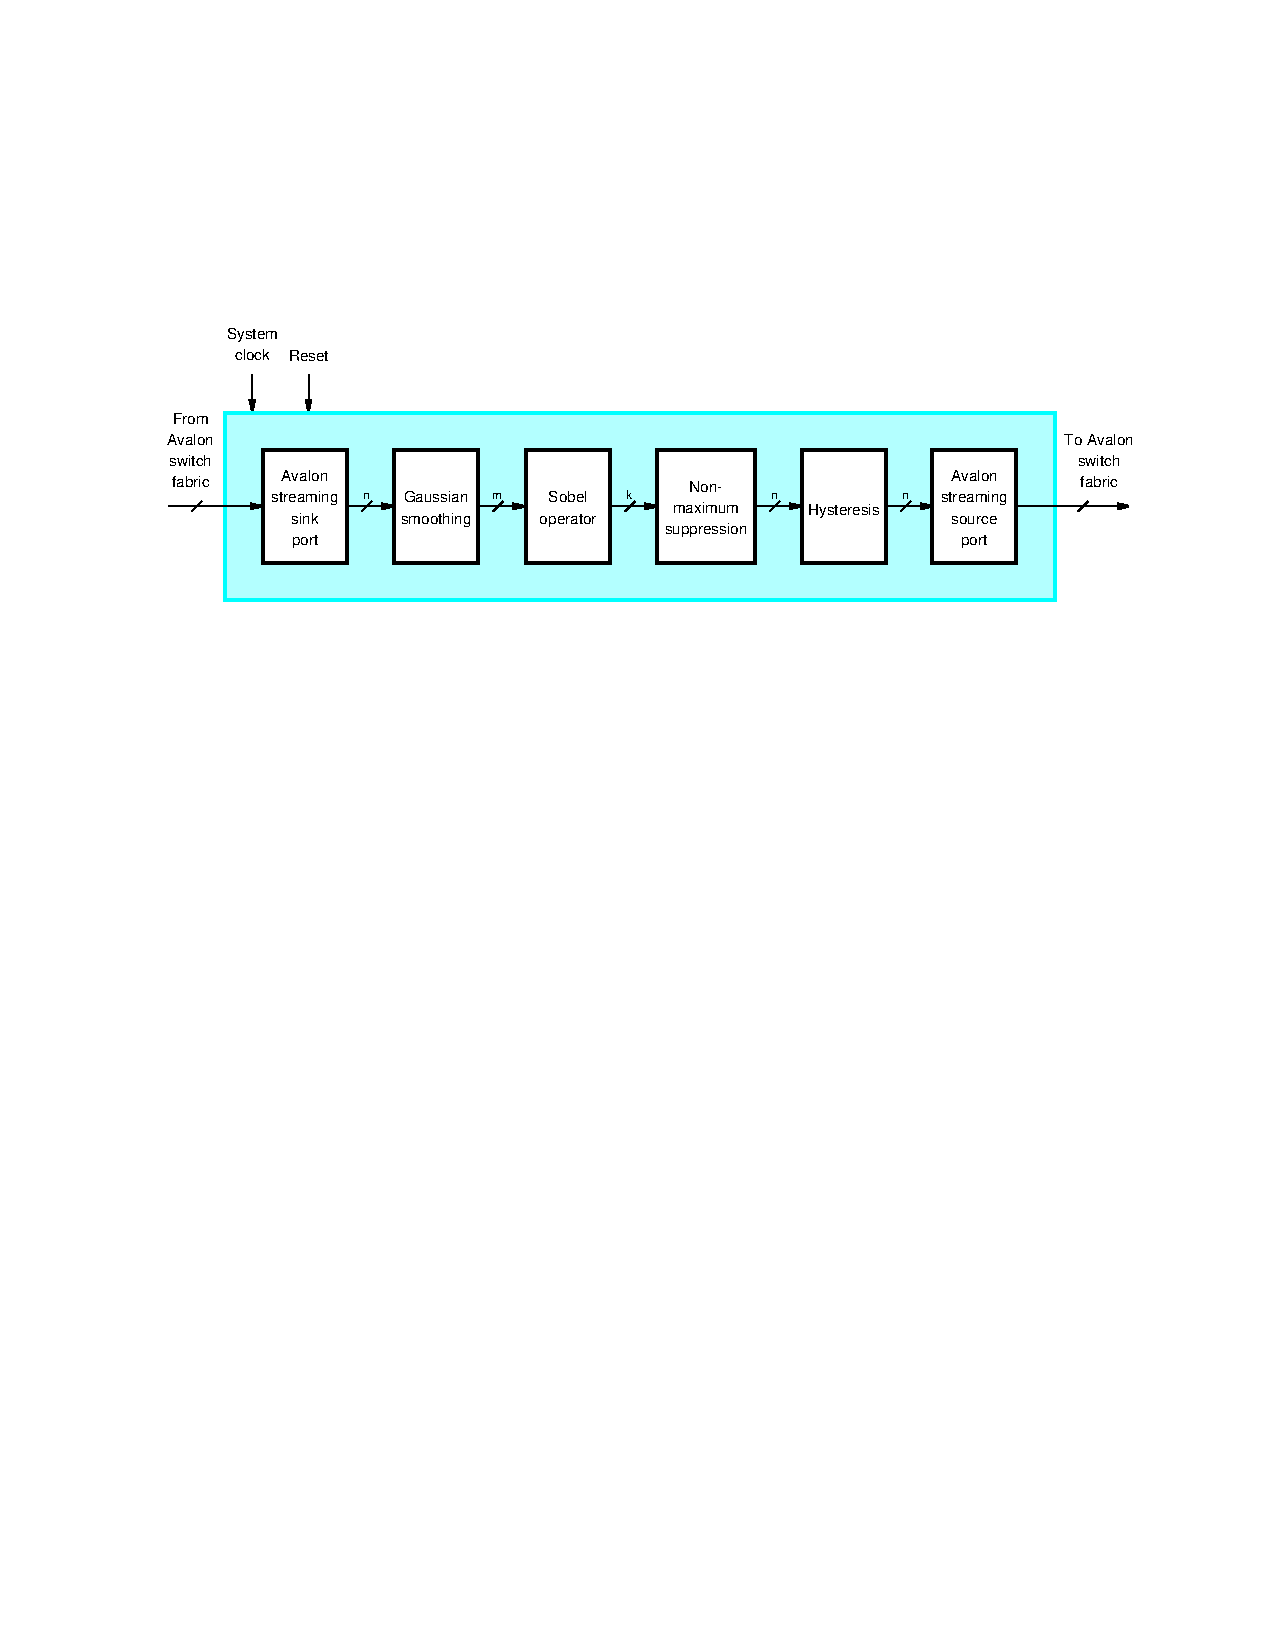
\includegraphics[width=0.8\textwidth]{figures/blockdiagram.pdf}
    \caption{Edge Detection}
    \label{fig:edgeDetection}
\end{figure}

\noindent
Figure \ref{fig:edgeDetection} is the block diagram of the Edge Detection IP core. The Edge Detection IP accepts streaming data with an Avalon-ST sink port, it then processes the data and passes the output to an Avalon-ST source port. We can add the Edge Detection IP to the streaming DMA system by connecting its Avalon-ST sink port to the Avalon-ST source port of the M2S DMA BBB, which will provide the source image as a serial stream, and its Avalon-ST source port to the Avalon-ST sink port of the S2M DMA BBB, which will store the result image in the processor's memory.\\
\\
Perform the following to add the Edge Detection IP to the streaming DMA system:
\begin{enumerate}
    \item Create a folder called \texttt{streaming\_dma\_system} and a within that a subfolder called \texttt{A10}. Copy the files in \texttt{hw/rtl/TEST\_streaming\_dma/A10} in {\it design\_files} accompanying this exercise to the \texttt{A10} folder, including a qsys file {\it streaming\_dma\_test\_system.qsys} and the folders \texttt{ip}, \texttt{QSYS\_IPs}, \texttt{stream\_to\_memory\_dma\_bbb} and \\ \texttt{memory\_to\_stream\_dma\_bbb}. 
    
    \item In the \texttt{streaming\_dma\_system} folder, create a Quartus project called \emph{streaming\_dma\_test\_system} and set \texttt{streaming\_dma\_test\_system.qsys} as the top-level design. Ensure you are using the same version of Quartus as exists on the DevCloud (19.2 most recently). Proper functionality is not guaranteed with a different version. 
    
    \item Open the {\it qsys} file in the Platform Designer. In \texttt{IP Catalog} , expand \texttt{Library} $\rightarrow$ \texttt{University Program} $\rightarrow$ \texttt{Audio \& Video} $\rightarrow$ \texttt{Video}, click on \texttt{Edge Detection} to create an instance of the \texttt{Edge Detection} IP core in the \emph{streaming\_dma\_test\_system}, setting the parameter \texttt{Width(\# of pixels)} to 720. Make the following connections:
        \begin{itemize}
            \item connect clk to dma\_clk.out\_clk
            \item connect reset to reset\_in.out\_reset
            \item connect avalon\_edge\_detection\_sink to m2s\_dma\_bbb.m2s\_st\_source
            \item connect avalon\_edge\_detection\_source to s2m\_dma\_bbb.s2m\_st\_sink
        \end{itemize}
        The resulting connections are shown in Figure \ref{fig:ip_connect}.
    
    \item Click the \texttt{Finish} button to save the qsys file for the streaming DMA system.
\end{enumerate}

\begin{figure}[h]
    \centering
    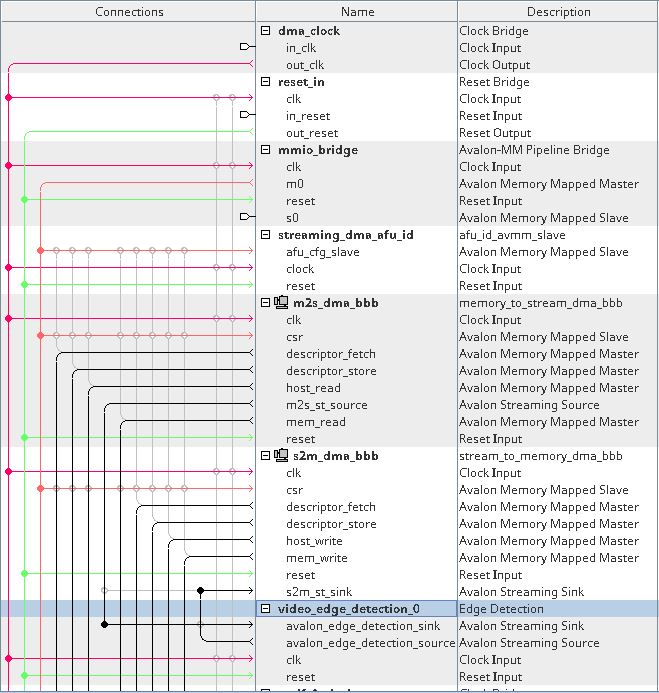
\includegraphics[width=0.6\textwidth]{figures/ip_connection.JPG}
    \caption{IP connection}
    \label{fig:ip_connect}
\end{figure}
Perform the following steps to complete the design of the AFU:
\begin{enumerate}
\item
Make a new folder on your home computer called \texttt{streaming\_dma\_afu}. Then, in this folder create two subfolders named \texttt{hw} and \texttt{sw}. The \texttt{sw} folder will be used in Part 2 of this exercise. Now, in the \texttt{hw} folder make a subfolder called \texttt{rtl}. This arrangement of folders is required when using the compilation tools that are provided on the DevCloud.

\item Copy the top-level file {\it afu.sv} to the \texttt{streaming\_dma\_afu/hw/rtl} folder. You also need to copy the files {\it ccip\_interface\_reg.sv}, {\it ccip\_std\_afu.sv} and the folders \texttt{BBB\_cci\_mpf} and \texttt{BBB\_ccip\_avmm} into the \texttt{rtl} folder. These files specify the CCI-P interface and convert it to the Avalon Memory Mapped interface for the DMA system.\\
\\
The development tools on the DevCloud also requires {\it filelist.txt}, which provides the path to all the design files for your AFU, and {\it streaming\_dma\_afu.json}, which gives some important information about the AFU. Copy the two files into the \texttt{rtl} folder.\\
\\
Copy the \texttt{streaming\_dma\_system} folder with your new DMA system to the \texttt{rtl} folder. Rename {\it streaming\_dma\_system} to {\it TEST\_streaming\_dma} to let the file paths aligned with those listed in {\it filelist.txt}.

\item Since the new DMA system has a new IP file for the \texttt{Edge Detection} component, we also need to list this file {\it filelist.txt}. Add the following path to {\it filelist.txt}:
\begin{lstlisting}
TEST_streaming_dma/A10/ip/streaming_dma_test_system/streaming_dma_test_system
_video_edge_detection_0.ip
\end{lstlisting}

\item
For the remainder of this exercise we assume that you are able to login to the DevCloud and configure the environment variables and settings that are needed for AFU development.  First, copy the folder \texttt{streaming\_dma\_afu} and its subfolders onto the DevCloud.  Then, 
using the Linux command line interface on the DevCloud execute the command 
\texttt{uuidgen} to generate a new UUID for the DMA AFU.
Enter this new UUID into the file \emph{streaming\_dma\_afu.json}, replacing the value of the key \emph{accelerator-type-uuid}.\\
\\
Update the parameter \emph{AFU\_ID\_H}  and \emph{AFU\_ID\_L} of \emph{streaming\_dma\_afu\_id.ip} to the upper 16 digits and lower 16 digits of the new UUID.  You must enter this in decimal, and you may use a calculator to make the conversion. For example, the UUID "633b3709-4b4a-415e-bddc-fd2e07e8d5e8" should be entered as: \emph{AFU\_ID\_H} = 7150369346438185310 and \emph{AFU\_ID\_L} = 13681088142187746792. The IP file is in \texttt{TEST\_streaming\_dma/A10/ip/streaming\_dma\_test\_system}.

\item
On the DevCloud, set your working directory to the \texttt{streaming\_dma\_afu} folder, and then 
run the command: 

\noindent
\texttt{afu\_synth\_setup -s hw/rtl/filelist.txt build\_synth}

Now, change your working directory to the newly-created \texttt{build\_synth} folder and 
execute the command \texttt{run.sh}. 
The \texttt{run.sh} command then executes the Intel 
Quartus\textsuperscript{\textregistered} Prime software to compile the AFU into a circuit
that can be implemented in the target FPGA device.

~\\
\noindent
The Quartus Prime software begins by executing its synthesis tools that
compile your Verilog source code. If any syntax errors are reported (they are shown in 
\red{red}), then fix these errors and compile again. 

~\\
\noindent
After successful compilation of your AFU code, the Quartus Prime software generates an FPGA 
programming bit-stream file called {\it dma\_afu.gbs}. You can download this {\it gbs} file into the FPGA device on the DevCloud by executing the command:

\noindent
\texttt{fpgasupdate streaming\_dma\_afu.gbs}.

Note that if you are using version 1.2.1 of the Arria 10 Development Stack on the
DevCloud, then you have to execute two commands to program the FPGA. First, execute:

\noindent
\texttt{PACSign PR -t UPDATE -H openssl\_manager -i streaming\_dma\_afu.gbs -o \\ streaming\_dma\_afu\_unsigned.gbs}

\noindent Type \texttt{y} ({\it yes}) in answer to the queries that are issued by this command. 
Then, execute:

\noindent
\texttt{fpgasupdate streaming\_dma\_afu\_unsigned.gbs}.
\end{enumerate}
~\\
\noindent
Now that the AFU has been downloaded into the target FPGA device, we can develop software 
programs which run on the processor and make use of the AFU.


\section*{Part II}
In this part of the exercise you are going to write a C program that utilizes the streaming DMA AFU for edge detection on an image. Figure \ref{fig:C_main} provides a template for the main function of your program. \\

\lstset{language=C,numbers=left,escapechar=\#}
\begin{figure}
\begin{center}
\begin{minipage}[h]{17.5 cm}
\begin{lstlisting}[name=C_code]
int main(int argc, char *argv[]) {
	fpga_result res = FPGA_OK;
	fpga_handle afc_h;
	fpga_dma_handle_t tx_dma_h, rx_dma_h;

	unsigned char * data;
	unsigned char * header;
	int width, height;
	if (read_grayscale(argv[1], &header, &data, &width, &height) < 0)  // read image
	    return -1;

	#\label{line:config}#struct config config = {
	    .data_size =  (uint64_t) width * height, 
	    .payload_size = std::stoi(argv[2])
	};
	                        
	#\label{line:open_AFU}#if(open_AFU(&afc_h) < 0) 
	    return -1;
	#\label{line:open_ST}#if(open_DMA_ST(afc_h, &rx_dma_h, &tx_dma_h) <0) 
	    return -1;

	struct buf_attrs battrs_src = { 	// source buffer
		.va = NULL,
		.iova = 0,
		.wsid = 0,
		.size = config.data_size
	};
	res = allocate_buffer(afc_h, &battrs_src);
	fill_buffer((unsigned char *)battrs_src.va, data, config.data_size);
	
	struct buf_attrs battrs_dst;            // dst buffer
	...
	
	// Host to FPGA transfer
	struct dma_config m2s_worker_struct;
	m2s_worker_struct.afc_h = afc_h;
	m2s_worker_struct.dma_h = tx_dma_h;
	m2s_worker_struct.config = &config;
	m2s_worker_struct.battrs = &battrs_src;
	m2s_worker_struct.image_header = header;

	pthread_t m2s_thread_id;  // m2s worker thread
	if (pthread_create(&m2s_thread_id, NULL, m2sworker, (void*)&m2s_worker_struct)!= 0) 
		return -1;
		
   // FPGA to host transfer
   struct dma_config s2m_worker_struct;    // config for fpga to host transfer
   pthread_t s2m_thread_id;                // s2m worker thread
    ...
    
	pthread_join(m2s_thread_id, nullptr);
	pthread_join(s2m_thread_id, nullptr);
	
	if(battrs_src.va)
		free_buffer(afc_h, &battrs_src);
	if(battrs_dst.va)
		free_buffer(afc_h, &battrs_dst);
	close_DMA_ST(rx_dma_h, tx_dma_h);
	close_AFU(afc_h);
	return 0;
}
\end{lstlisting}
\end{minipage}
\caption{Using the AFU in a C program}
\label{fig:C_main}
\end{center}
\end{figure}

\noindent
In Line \ref{line:config}, the code initializes a \emph{config} struct for the DMA transfer. \emph{data\_size} is the total size of the data to transfer and \emph{payload} is the size of data transferred each time. The AFU transfers a block of data of \emph{payload} size using one or more DMA transfers and signals the processor when the entire block is transferred. We set the \emph{data\_size} to the size of the image and pass in \emph{payload} as an argument.\\
\\
In Line \ref{line:open_AFU}, the code calls \emph{open\_AFU} to set up the communication between the program and the AFU.  In Line \ref{line:open_ST}, the function {\it open\_DMA\_ST} searches for the S2M and M2S DMA BBBs in the AFU and counts the number of the DMA BBBs ({\it channels}) that the program can access. It then sets up separate handles for each channel. The handles are later used in separate threads to control data transfers.\\
\\
The code then allocates a buffer to store the source image in the shared memory. The {\it buf\_attrs} struct includes the address of the allocated buffer in the processor's view ({\it va}),  the address of the buffer in the DMA's view ({\it iova}) and the handle to the buffer to be used with other functions ({\it wsid}), which are set by the {\it allocate\_buffer} function.\\


\noindent
To send and receive data at the same time, the code launches two threads. The m2s thread transfers data from the processor to the AFU while the s2m thread transfers data from the AFU to the processor. A {\it dma\_config} struct needs to be instantiated for each thread to pass in the handles of the AFU, the transfer configuration and the information of the shared-memory buffer to store data.\\
~\\
Figure \ref{fig:m2sworker} shows the code of the \emph{m2sworker} function. It first initializes a handle \emph{transfer} for the memory-to-stream transfers (Line \ref{line:transfer_init}) and resets the attributes of the handle to default values (Line \ref{line:transfer_reset}). The code then utilizes the \emph{transfer} handle to set up transfers. One payload (block of data of \emph{payload} size) is transferred at a time. \\
\\
Line \ref{line:transfer_src} to \ref{line:transfer_last} set the attributes for a memory-to-stream {\it transfer}, which includes a source address ({\it Src}), a destination address ({\it Dst}) and the length of the data to transfer ({\it Len}). A memory-to-stream transfer also includes a transfer type specifying the direction of the transfer. Since the TX DMA is used for transferring data from memory to stream, we also need to set the {\it TXControl} attribute, which specifies whether to generate a Start-of-Packet(SOP) or an End-of-Packet(EOP) signal. For this lab, we set {\it TXControl} to \verb|TX_NO_PACKET| (not generate SOP or EOP) for all the transfers. For efficiency, all transfers are done asynchronously and we define a call back function {\it mtosCb} to keep track of the completion of the transfers. It's also required to indicate whether a payload is the last piece of data in the buffer. This is done by the OPAE function {\it fpgaDMATransferSetLast}. \\

\noindent
Perform the following steps to complete the C program: 
\begin{enumerate}
    \item Complete the code for the {\it main} function in {\it edge\_detect.cpp} in \texttt{design\_files/sw} included along with this exercise. You need to allocate a buffer in the shared memory to store the result image and create a thread for transferring data from the AFU to the processor.
    
    \item Complete the code for the {\it s2mworker} function in {\it fpga\_dma\_st\_test\_utils.cpp}. Figure \ref{fig:s2mworker} provides a template for this function. Similar to {\it m2sworker}, it should first initialize a handle for the transfers, and then transfer one payload at a time. The code then waits for the transfers to complete. After all transfers are done, the function should write the result image to a {\it .bmp} file.\\
    \\
    The {\it src} address of a transfer should be 0 while the {\it dst} address should be based on the address of the shared-memory buffer in the DMA's view ({\it dma\_config} $\rightarrow$ {\it battrs} $\rightarrow$ {\it iova}). The transfer types are listed in the enum object {\it fpga\_dma\_transfer\_type\_t} in the header file {\it fpga\_dma\_types.h}. You should set the \texttt{TransferType} for each transfer to \verb|FPGA_ST_TO_HOST_MM|. For this lab, we receive a fixed length (size of image) of data, so we set the RX control to \verb|RX_NO_PACKET| for all transfers and indicate whether a transfer is the last one with the function {\it fpgaTransferSetLast}.
    \item Copy the files in \texttt{design\_files/sw} to the \texttt{streaming\_dma\_afu/sw} directory on the Devcloud. Run \verb|make| to compile your program. To execute your program type \verb|./edge_detect [payload] [path to image]|.\\
    \\
    Note that the image needs to have a width of 720 pixels, which is set by the parameter of the \texttt{Edge\_Detection} IP. Three images is provided for you in \texttt{design\_files/images}.
    
    \item A Perl file {\it profile} is provided for you in \verb|design_files/sw|. It runs the software program with different payload size and create a table of the transfer bandwidth and time against the payload size.\\
    \\
    Time the part of your main function that does data transfer and add the following lines after the pthreads join in your main function:
\lstset{language=C, numbers=none, escapechar=|}
\begin{lstlisting}
std::cout << "Memory to Stream BW = " << m2s_worker_struct.bw << " MBps, " \
			  << "Stream to Memory BW = " << s2m_worker_struct.bw << " MBps, " \
			  << "Time = " << time << " s" << endl;
\end{lstlisting}
    Run the Perl file by typing \verb|./profile|. A sample output is shown in Figure \ref{fig:output}.

\lstset{language=C,morekeywords={u42132@s005-n005,LFSR},numbers=none,escapechar=|}
\begin{figure}[h]
\begin{center}
\begin{minipage}[h]{\textwidth}
\begin{lstlisting}[name=output]
|\green{userid@s005-n007}:\blue{~/streaming\_dma\_afu/sw}|$ ./profile
Total data size = 388800 bytes
-----------------------------------------------
payload         mtos    stom    time
-----------------------------------------------
64B             45      44      0.0691999
128B            113     115     0.0210434
256B            192     189     0.0203319
1024B           195     189     0.0229187
2KB             187     177     0.0202809
4KB             190     188     0.0205957
16KB            185     184     0.0266839
64KB            187     184     0.0202029
256KB           192     189     0.0233965

|\green{userid@s005-n007}:\blue{~/streaming\_dma\_afu/sw}|$
\end{lstlisting}
\end{minipage}
\caption{Executing \texttt{./profile}}
\label{fig:output}
\end{center}
\end{figure}
    
\end{enumerate}


\lstset{language=C,numbers=left,escapechar=\#}
\begin{figure}
\begin{center}
\begin{minipage}[h]{17.5 cm}
\begin{lstlisting}[name=C_mtos]
volatile static uint64_t bytes_sent;

static void mtosCb(void *ctx, fpga_dma_transfer_status_t status) {
	bytes_sent += status.bytes_transferred;
}

void * m2sworker(void* arg) {
	struct timespec start, end;
	struct dma_config *dma_config = (struct dma_config *)arg;
	struct config *test_config = dma_config->config;
	fpga_result res = FPGA_OK;

	// initialize DMA transfer
	fpga_dma_transfer_t transfer;
	#\label{line:transfer_init}#res = fpgaDMATransferInit(&transfer);
	if(res != FPGA_OK){
		fprintf(stderr, "Error: allocating m2s transfer\n");
		return dma_config->dma_h;
	}
	#\label{line:transfer_reset}#fpgaDMATransferReset(transfer);

	// do memory to stream transfer
	size_t total_size = test_config->data_size;
	uint64_t max = ceil((double)test_config->data_size / (double)test_config->payload_size);
	uint64_t tid = 0; // transfer index
	uint64_t src = dma_config->battrs->iova;
	bytes_sent = 0;
	clock_gettime(CLOCK_MONOTONIC, &start);
	
	while(total_size > 0) {
		uint64_t transfer_bytes = MIN(total_size, test_config->payload_size);
		#\label{line:transfer_src}#fpgaDMATransferSetSrc(transfer, src);
		fpgaDMATransferSetDst(transfer, (uint64_t)0);
		fpgaDMATransferSetLen(transfer, transfer_bytes);
		fpgaDMATransferSetTransferType(transfer, HOST_MM_TO_FPGA_ST);
		fpgaDMATransferSetTxControl(transfer, TX_NO_PACKET);
		fpgaDMATransferSetTransferCallback(transfer, mtosCb, NULL);
		if(tid == max-1) { // last transfer
			fpgaDMATransferSetLast(transfer, true);
		} else {
			fpgaDMATransferSetLast(transfer, false);
		#\label{line:transfer_last}#}
		// do transfer
		res = fpgaDMATransfer(dma_config->dma_h, transfer);
		if(res != FPGA_OK){
			fprintf(stderr, "Error: m2s transfer error\n");
			fpgaDMATransferDestroy(&transfer);
			return dma_config->dma_h;
		}
		total_size -= transfer_bytes;
		src += transfer_bytes;
		tid++;
	}
	
	while(bytes_sent < test_config->data_size);

	clock_gettime(CLOCK_MONOTONIC, &end);
	dma_config->bw = getBandwidth(test_config->data_size, getTime(start,end));
	res = fpgaDMATransferDestroy(&transfer);
	return dma_config->dma_h;
}
\end{lstlisting}
\end{minipage}
\caption{Host to FPGA transfer}
\label{fig:m2sworker}
\end{center}
\end{figure}


\lstset{language=C,numbers=left,escapechar=\#}
\begin{figure}
\begin{center}
\begin{minipage}[h]{17.5 cm}
\begin{lstlisting}[name=C_stom]
volatile static uint64_t bytes_rcvd;

static void stomCb(void *ctx, fpga_dma_transfer_status_t status) {
	bytes_rcvd += status.bytes_transferred;
}

void * s2mworker(void* arg) {
	struct timespec start, end;
	struct dma_config *dma_config = (struct dma_config *)arg;
	struct config *test_config = dma_config->config;
	
	fpga_result res = FPGA_OK;	
	
	fpga_dma_transfer_t transfer;
    // initialize the transfer handle
    ...

	bytes_rcvd = 0;
	uint64_t transfer_bytes;
	size_t total_size;
	uint64_t tid;
	uint64_t dst;

	clock_gettime(CLOCK_MONOTONIC, &start);

	while(total_size > 0) {
		// set up the attributes of a transfer
		...
		
		res = fpgaDMATransfer(dma_config->dma_h, transfer);
		
		...
	}

	while(bytes_rcvd < expected_bytes);
	
	clock_gettime(CLOCK_MONOTONIC, &end);
	dma_config->bw = getBandwidth(test_config->data_size, getTime(start,end));

	// write result image
	write_grayscale_bmp("edges.bmp", (unsigned char *)dma_config->image_header, (unsigned char *)dma_config->battrs->va);

	res = fpgaDMATransferDestroy(&transfer);
	return dma_config->dma_h;
}
\end{lstlisting}
\end{minipage}
\caption{FPGA to Host transfer}
\label{fig:s2mworker}
\end{center}
\end{figure}

%%%%%%%%%%%%%%%%%%%%%%%%%%%%%%%%%%%%%%%%
%%% FPGAcademy Copyright Information %%%
%%%%%%%%%%%%%%%%%%%%%%%%%%%%%%%%%%%%%%%%

%Always put the copyright on a new page (clear page), with some vertical space from top
\clearpage
\vspace{1in}

\noindent

Copyright {\copyright} FPGAcademy.org. All rights reserved. FPGAcademy and the 
FPGAcademy logo are trademarks of FPGAcademy.org.  This document is provided 
"as is", without warranty of any kind, express or implied, including but not 
limited to the warranties of merchantability, fitness for a particular purpose 
and noninfringement. In no event shall the authors or copyright holders be 
liable for any claim, damages or other liability, whether in an action of 
contract, tort or otherwise, arising from, out of or in connection with the 
document or the use or other dealings in the document.
~\\
~\\
**Other names and brands may be claimed as the property of others.



\end{document}
